\chapter{Алгебра и геометрия. \\ \hfill Линейная алгебра}

\begin{multicols}{2}
\raggedcolumns 

\section{Группы, кольца, поля. Определения и примеры. Циклические группы. Теорема о гомоморфизме}

\begin{definition}{(Группа)}{}
    Непустое множество $\mathcal{G}$, на котором определена некая операция $\bullet: \mathcal{G} \times \mathcal{G} \to \mathcal{G}$, называется группой, если выполнены 3 свойства: $(\forall a,b,c \in \mathcal{G})$
    \begin{enumerate*}
        \item ассоциативность $a\bullet(b\bullet c) = (a\bullet b)\bullet c$;
        \item существование нейтрального элемента $\exists e \in \mathcal{G}: e\bullet a = a\bullet e = a$;
        \item существование обратного элемента $\exists a^{-1}\in \mathcal{G} : a\bullet a^{-1} = a^{-1}\bullet a = e\in \mathcal{G}$;
    \end{enumerate*}  
\end{definition}
Если $(\mathcal{G}, \bullet)$ удовлетворяет только свойству 1., то множество называется полугруппой. Если свойства 1. и 2., то моноид.
Пример: 
\begin{multicols}{2}
    \begin{enumerate*}
    \item $\left(\Z, +\right)$ -- группа;
    \item $\left(\Z, \cdot\right)$ -- моноид;
    \item $\left(\Q\backslash \left\{0\right\}\right)$ -- группа;
    \item $\left(\R, +\right)$ -- группа;
    \item $\left(\R \backslash \{0\}\right)$ -- группа.
\end{enumerate*}
\end{multicols}
\begin{note}
    Абелевой группой называется группа $(\mathcal{G}, \bullet)$ в соответствии с определением, но обладающая также коммутативностью: \[\forall a,b \in \mathcal{G} \ ab = ba\]
\end{note}
Примеры:
\begin{multicols}{2}
\begin{enumerate*}
    \item $(V_{2,3})$ -- группа;
    \item $(M_{n\times k}, +)$ -- группа;
    \item $(M_{n\times n}, \cdot)$ -- моноид;
    \item $S_n = \{\sigma: \{1, \ldots, n\} \to \\ \to \{1, \ldots, n\}\}$ -- симметричная группа, но не абелева. Группа перестановок. Операция -- композиция. 
\end{enumerate*}
\end{multicols}
\begin{definition}{(Кольцо)}{}
    Множество $R$ с двумя бинарными операциями $+$ и $\bullet$, для которого справедливы свойства:
    \begin{enumerate*}
        \item Абелева группа по сложению $(R, +)$;
        \item Моноид по умножению $(R, \bullet)$;
        \item Дистрибутивность относительно умножения и сложения $\forall a,b,c \in R$:
        \[
            \begin{array}{c}
                a(b+c) = ab+ac\\
                (a+b)c = ac+bc
            \end{array}
        \]  
    \end{enumerate*} 
\end{definition}
Кольцо коммутативно, если умножение коммутативно.
Примеры:
\begin{multicols}{2}
    \begin{enumerate*}
        \item $\Z, \Q, \R$ -- кольца (коммутативные);
        \item $M_n(\R)$ -- кольцо;
        \item $2\Z$ (четные числа) -- кольцо с единицей;
        \item $(R^{*}, \bullet)$ -- группа (множество всех обратимых элементов кольца);
        \item $\Q^*=\Q\backslash\{0\}, \Z^* = \{\pm 1\}$
    \end{enumerate*}
\end{multicols}
\begin{definition}{(Поле)}{}
    Коммутативное кольцо $R$ называется полем, если его мультипликативная группа \mbox{$R^* = R\backslash \{0\}$}
\end{definition}
Примеры: $\Q, \R, \C$ -- поле, $\Z$ -- кольцо, но не поле.
\begin{definition}{(Изоморфизм)}{}
    Пусть $M$ -- множество с операцией $\circ$, а $N$ -- множество с операцией $\bullet$. Алгебраические структуры $(M, \circ)$ и $(N, \bullet)$ называются изоморфными ($(M, \circ) \simeq (N, \bullet)$), если существует биективное отображение\useshortskip \[
            f: \ M \to N
        \]
    такое, что ($\forall a,b \in M$):\useshortskip
    \[
        f(a\circ b) = f(a) \bullet f(b)
        \]
    $f$ в таком случае называют изоморфизмом структур $(M, \circ)$ и $(N, \bullet)$.
\end{definition}
Пример: $a \to 2^a$ -- изоморфизм множества $\R$ с операциями сложения и множества положительных чисел с операцией умножения $(2^{a+b} = 2^a2^b)$.
\bigskip
\par

Пусть $M$ -- множество с операцией $\bullet$ и $N$ -- какое-либо его подмножество. Говорят, что $N$ замкнуто относительно операции $\bullet$, если:\useshortskip
\[
    a,b\in N: \ a \bullet b \in N
    \]
\begin{definition}{(Подгруппа)}{}
    Подмножество $B$ абелевой группы (аддитивной) $A$ называется подгруппой, если:
    \begin{enumerate*}
        \item $B$ замкнуто относительно сложения;
        \item $a\in B \Longrightarrow -a \in B$;
        \item $0 \in B$.
    \end{enumerate*}
\end{definition}
\begin{note}{}{}
    Для мультипликативной группы подмножество $B$ будет называться подгруппой, если:
    \begin{enumerate*}
        \item $B$ замкнуто относительно умножения;
        \item $a\in B \Longrightarrow a^{-1} \in B$;
        \item $e \in B$.
    \end{enumerate*}
    В аддитивной абелевой группе $\R$ справедлива цепочка:\useshortskip
    \[
        \Z \subset \Q \subset R
        \]
    В мультипликативной группе $\R^*$:\useshortskip
    \[
        \Z^* = \{\pm 1\} \subset \Q^{*} = \Q\backslash \{0\} \subset \R^*.
        \]
\end{note}
\begin{definition}{(Подкольцо)}{}
    Подмножество $L$ кольца $K$ называется подкольцом, если 
    \begin{enumerate*}
        \item $L$ является подгруппой аддитивной группы кольца $K$;
        \item $L$ замкнуто относительно умножения.
    \end{enumerate*}
\end{definition}
Подкольцо само является кольцом. Цепочка подгрупп аддитивной группы $\R$ является и цепочкой подколец.
\begin{definition}{(Подполе)}{}
    Подмножество $L$ поля $K$ называется подполем, если 
    \begin{enumerate*}
        \item $L$ является подкольцом кольца $K$;
        \item $a\neq 0\in L \Longrightarrow a^{-1} \in L$;
        \item $e \in L.$
    \end{enumerate*}
\end{definition}
Поле $\Q$ -- подполе поля $\R$.
\par
Порядок группы -- это $|\mathcal{G}|$
\subsection*{Еще примеры групп}
\begin{enumerate*}
    \item $GL_n(F) = M_n(F)^* = \{A \in M_n (F): \ |A| \neq 0\}$;
    \item $SL_n(F) = \{A \in GL_n(F):\ |A| = 1\} \subseteq GL_n(F)$;
    \item $T_n(F) = \{A = [a_{ij}] \in GL_n(F): \ a_{ij} = 0 \ \forall i,j: i>j\} \subseteq GL_n(F)$;
    \item $GL_n(\Z) = M_n(\Z)^*$;
    \item $S_n$ -- группа перестановок на $n$ элемента $x$:
    \[
        S_n = \{\sigma: \ [n] \to [n] -- \text{ биекция}\}
        \]
\end{enumerate*}
\begin{definition}{(Гомоморфизм)}{}
    Гомоморфизмом группы $\mathcal{G}$ в группу $\mathcal{H}$ называют отображение $f: \mathcal{G} \to \mathcal{H}$, удовлетворяющее условию:\useshortskip
    \[f(ab) = f(a)f(b)\]
\end{definition}
\subsubsection*{Примеры гомоморфизма}
\begin{enumerate*}
    \item $(-1)^{\sigma\tau} = (-1)^\sigma (-1)^\tau$
    \par Это свойство говорит, что есть гомоморфизм $\mathrm{sgn}: S_n \to \Z^* = \left(\{\pm 1\}\right)$
    \[
        \mathrm{sgn} (\sigma \tau) = \mathrm{sgn}\sigma \cdot \mathrm{sgn} \tau
        \]
\end{enumerate*}
\begin{theorema}{(Кэли)}{}
    Пусть $\mathcal{G}$ -- группа, $|\mathcal{G}| = n$. Тогда в $S_n$ есть подгруппа $H \subseteq S_n, \ H \cong \mathcal{G}$
\end{theorema}
\begin{theorema}{(О гомоморфизме групп)}{}
    Пусть $f: \mathcal{G} \to \mathcal{H}$ -- гомоморфизм групп. Тогда\useshortskip
    \[\im f \simeq \mathcal{G}\ker f\] 
    Или имеется изоморфизм:\useshortskip
    \[\varphi: \ \im f \cong \mathcal{G}/\ker f\]
\end{theorema}
\section{Подстановки. Определение подстановки, четность подстановок. Произведение подстановок, разложение подстановок в произведение транспозиций и независимых циклов.}
\begin{definition}{(Циклическая группа)}{}
    Группа $\mathcal{G}$ называется циклической, если $\exists g \in G: \ G = <g>$
\end{definition}
$\Z, \ \Z_n$ -- циклические группы.
\begin{definition}{(Порядок)}{}
    Пусть $a\in G$. Тогда порядок элемента $a$ ($\ord a$) -- это наименьшее натуральное $n$: \ $a^n = e$. Если такого $n$ нет, то $\ord a = \infty.$
\end{definition}
\textbf{Пример:} В $\Z_n \ \ord 1 = n$.
\begin{proposition}{}{}
    Пусть $a\in \mathcal{G}, \ \ord a = n$. Тогда $\forall k \in \Z, \ a^k = e \Longleftrightarrow n|k.$
\end{proposition}
\begin{proposition}{}{}
    $\ord a = |<a>|.$
\end{proposition}
\begin{definition}{(Перестановка)}{}
    Перестановка на $n$ элементах -- это биекция $\sigma : [n] \to [n]$, где $[n] = \{1 , \ldots, n\}$. Множество всех перестановок -- $S_n$. 
\end{definition}
$S_n$ -- группа относительно операции композиции:
\[
    \sigma \cdot \tau = \sigma \circ \tau: [n]\to [n], \ \sigma \circ \tau(i) = \sigma(\tau(i))  
\]
Табличный вид записи перестановки:
\[
    \sigma = \begin{pmatrix}
        1 & 2 & \ldots & n\\
        \sigma(1) & \sigma(2) & \ldots & \sigma(n)
    \end{pmatrix}
\] 
Цикл: $\sigma = (i_1, i_2, \ldots, i_k) \in S_n$ -- перестановка, которая $\sigma(i_s) = i_{s+1},\ s=1, \ldots, k-1, \ \sigma(i_k) = i_1$, а остальные элементы $[n]$ неподвижны ($\sigma(x) = x$).
\begin{definition}{(Независимость циклов)}{}
    Циклы $\sigma = (i_1, \ldots, i_k), \ \tau = (j_1, \ldots, j_l)$ независимы, если:
    \[
        \{i_1, \ldots, i_k\} \cap \{j_1, \ldots, j_l\} = \emptyset.    
    \]
\end{definition}
Для независимых циклов естественна коммутативность.
\begin{proposition}{}{}
    Любая перестановка $\sigma \in S_n$ представима в виде произведения нескольких независимых циклов.
\end{proposition}
Построим это разложение. Будем записывать циклы вида $(i)$, если $\sigma(i) = i$. Когда-то в списке $i_1, i_2, \ldots$ появится повтор. Первым повторится $i_1$, иначе $i_{k+1} = \sigma(i_k) = i_s = \sigma(i_{s-1})$. Тогда $i_k = i_{s-1}$. Противоречие. Получили первый цикл. У каждого элемента в цикле там же содержится его $\sigma$ - образ и $\sigma$ -- прообраз. Выберем наименьшее из $[n]$, которое еще не в цикле $j_1$ и повторим процедуру. Аналогично получим второй цикл и так далее. В итоге получим, что $\sigma (i_1, \ldots, i_k)(j_1, \ldots, j_l)\ldots$
\begin{definition}{(Транспозиция)}{}
    Транспозиция -- цикл длины 2, т.е. перестановка вида $(i,j), \ i\neq j.$
\end{definition}
\begin{proposition}{}{}
Каждая перестановка $\sigma \in S_n$ есть произведение нескольких транспозиций.
\end{proposition}
Индукция по $n$. При $n=1$ (id -- пустое произведение). Пусть $\sigma \in S_n$, если $\sigma(n) = n$, то $\sigma \in S_{n-1}$. Для нее предположение верно по индукции. Если $\sigma(n) = i$, то положим $\tau = (i,n)\sigma$, тогда $\tau(n) = n \Rightarrow \tau$ -- произведения транспозиций и $\sigma = (i,n)^{-1}\tau = (i, n)\tau$.
\begin{definition}{(Инверсия)}{}
    Пусть $\sigma\in S_n$. Назовем беспорядком (инверсией) в перестановке $\sigma$ такую пару $(i,j): \ 1 \leq i < j \leq n, \ \sigma(i) > \sigma(j)$. Обозначим $N(\sigma)$ -- число беспорядков в $\sigma$. Знак $\sigma: \ \mathrm{sgn} \sigma = (-1)^\sigma := (-1)^{N(\sigma)}$.
\end{definition}
Если $(-1)^\sigma = 1$, то $\sigma$ -- четная, иначе нечетная.
\section{Комплексные числа. Геометрическое изображение, алгебраическая и тригонометрическая форма записи, извлечение корней, корни из единицы.}
Аксиоматическое определение поля комплексных чисел.
\begin{definition}{(Поле $\C$)}{}
    Полем комплексных чисел называется всякое поле $\C$, обладающее следующими свойствами:
    \begin{enumerate*}
        \item оно включает в себя подполе $\R$;
        \item $i \in \C: \ i^2 = -1$;
        \item минимально среди полей с предыдущими свойствами, т.е. $K \subset \C: K \ni \R, i \Longrightarrow K = \C.$
    \end{enumerate*}
\end{definition}
Теорема о единственности поля $\C$ и алгебраическая форма представления. $a (\im)$ -- вещественная часть, $b (\re)$ -- мнимая.
\begin{theorema}{(Единственность поля $\C$)}{}
    Поле комплексных чисел существует и единственно с точностью до изоморфизма, переводящего $\R \to \C$. Каждое комплексное число представляется в виде $a+bi, \ a,b\in \R, \ i: \ i^2 = -1$.
\end{theorema}
Рассмотрим изоморфизм вида:\useshortskip
\[
    f: \ \C \to \C, \hspace*{0.5cm} c=a+bi \to \overline{c} = a-bi', \hspace*{0.5cm} (a,b\in\R)
    \]
\par
Такое отображение называется комплексным сопряжением. Любой изоморфизм любой алгебраической структуры на себя называется автоморфизмом.
\begin{wrapfigure}{r}{0.5\columnwidth}
    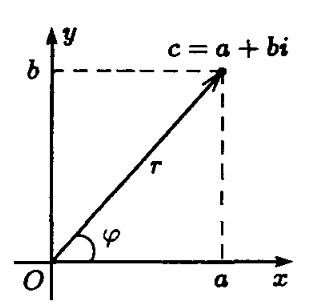
\includegraphics[scale=0.65]{images/complex_field_trigonometric.png}
    \caption{Геометрическое изображение комплексного числа.}
    \label{fig:complex_field}
\end{wrapfigure}
Комплексные числа можно изображать точками или векторами на плоскости. Число $c=a+bi$ изображается точкой или вектором с декартовыми координатами $(a,b)$.
Модулем комплексного числа $c=a+bi$ называется длина вектора, изображающего это число. Модуль при этом равен:\useshortskip
\[
    |c| = \sqrt{a^2 + b^2}
    \]
\par
Аргумент ($\arg c$) -- угол, между вектором и положительным направлением оси. Аргумент числа 0 не определен.
$r$ и $\varphi$ -- модуль и аргумент числа $c$. Тогда получим, что \[a=r\cos \varphi, \hspace*{0.5cm} b = r\sin \varphi\]
Тогда (тригонометрическое представление)
\[
    c = r(\cos \varphi + i\sin \varphi)
    \]
Формулы для умножения, деления и возведения в степень:
\[
    \begin{array}{c}
        r_1(\cos \varphi_1 + i\sin\varphi_1)\cdot r_2(\cos \varphi_2 + i\sin \varphi_2) = \\ = r_1r_2(\cos(\varphi_1 + \varphi_2) + i\sin(\varphi_1 + \varphi_2))\\[0.5cm]
        \dfrac{r_1(\cos\varphi_1 + i\sin\varphi_1)}{r_2(\cos\varphi_2 + i\sin\varphi_2)} = \\ = \dfrac{r_1}{r_2}\left(\cos\left(\varphi_1-\varphi_2\right) + i\sin\left(\varphi_1 - \varphi_2\right)\right)\\[0.5cm]
        \left[r(\cos\varphi + i\sin\varphi)\right]^n = r^n(\cos n\varphi + i\sin n\varphi)\\(\text{формула Муавра})
    \end{array}
    \]
Извлечение корня $n$-й степени из комплексного числа \mbox{$c = r(\cos\varphi + i\sin\varphi)$} есть решение уравнения $z^n = c$. Пусть $|z| = s, \arg z = \psi \Rightarrow s^n = r,\ n\psi = \\ = \varphi + 2\pi k \ (k\in\Z)$. Имеем $s = \sqrt[n]{r}, \ \psi = \dfrac{\varphi + 2\pi k}{n}$:
\[
    z = \sqrt[n]{r} \left(\cos\dfrac{\varphi+2\pi k}{n} + i\sin \dfrac{\varphi + 2\pi k}{n}\right)
    \]
\begin{note}{}{}
    Корень $z = i$. Имеем $|z| = 1, \ \arg z = \dfrac{\pi}{2}$
    \[
        \sqrt{i} = \cos\dfrac{\dfrac{\pi}{2}+2\pi k}{2} + i\sin\dfrac{\dfrac{\pi}{2} + 2\pi k}{2}, \ k = 0,1.
        \]
\end{note}
\section{Системы линейных уравнений. Прямоугольные матрицы. Приведение матриц и систем
линейных уравнений к ступенчатому виду. Метод Гаусса.}
Системы линейных уравнений -- системы вида:
\[
    \left\{\begin{array}{c}
        a_{11}x_1 + a_{12}x_2 + \ldots + a_{1n}x_n = b_1,\\
        a_{21}x_1 + a_{22}x_2 + \ldots + a_{2n}x_n = b_2,\\
        \vdots\\
        a_{k1}x_1 + a_{k2}x_2 + \ldots + a_{kn}x_n = b_k.
    \end{array}\right.
    \]
При этом $a_{ij} \in F, \ b_j \in F$. Система имеет матричный вид $Ax=b$, где:
\[
    A = \begin{bmatrix}
        a_{11} &\ldots & a_{1n}\\
        \vdots & \ddots & \vdots\\
        a_{k1} & \ldots & a_{kn}
    \end{bmatrix} \in M_{k\times n}(F), \hspace*{0.5cm} b = \begin{bmatrix}
        b_1\\\vdots\\b_k
    \end{bmatrix} \in F^k
    \]
Решить систему -- найти все $x = \begin{bmatrix}
    x_1 \\\vdots \\x_k
\end{bmatrix} \in F^n$, удовлетворяющие $Ax=b$. Введем понятия:
\begin{itemize}
    \item[] расширенная матрица СЛУ: $[A | b]$;
    \item[] однородное СЛУ: $b = 0$;
    \item[] СЛУ совместна: есть хотя бы одно решение;
    \item[] Две СЛУ $A_1x = b, \ A_2x=b_2$ эквивалентны $A_1x_0 = b_1 \Longleftrightarrow A_2x_0 = b_2$.
\end{itemize}
Рассмотрим совместную систему $Ax=b$. Пусть $x_0$ -- частное решение $(Ax_0 = b)$, $U$ -- подпространство решений ОСЛУ $Ax=0$, тогда множество решений исходной системы это \useshortskip
\[
    x_0 + U = \{x_0 + u:\ u \in U\}
    \]
\begin{definition}{(Преобразования матриц)}{}
    Элементарные преобразования -- преобразования трех типов:\vspace*{0.3cm}

        \small{\begin{tabular}{|p{.25\columnwidth}|p{.33\columnwidth}|p{.3\columnwidth}|}
            \hline
            \footnotesize{Элем. пр-ния} & \footnotesize{Элем. матрицы} & \footnotesize{Обратные} \\\hline
            1) К одной строке прибавить другую, умноженную на скаляр & $D_{ij}(\alpha) = E + \alpha \cdot E_{ij}$\vspace*{-0.1cm} \[ \scriptstyle \hspace*{0.1cm} \begin{bmatrix} \scriptstyle
                1& \scriptstyle 0 &\scriptstyle \ldots & \scriptstyle \ldots & \mypoint{here1}{\scriptstyle0}\\ \scriptstyle \vdots &\scriptstyle 1 &\scriptstyle \ddots & \scriptstyle\vdots & \scriptstyle\vdots\\
                \scriptstyle \mypoint{here2}{\scriptstyle 0} & \scriptstyle\ldots & \scriptstyle1 & \scriptstyle \ldots & \scriptstyle \alpha\\
                \scriptstyle\vdots & \scriptstyle\ldots  & \scriptstyle\ldots & \scriptstyle\ddots & \scriptstyle0\\
                \scriptstyle 0& \scriptstyle\ldots & \scriptstyle\ldots & \scriptstyle\ldots & \scriptstyle 1
            \end{bmatrix}\begin{tikzpicture}[remember picture, overlay]
                \node[above=5pt of here1](textofhere1){\scriptsize j};
                \draw[myarrow] (textofhere1) -- (here1);
                \node[left=6pt of here2](textofhere2){\scriptsize i};
                \draw[myarrow] (textofhere2) -- (here2);
              \end{tikzpicture}\] & $D_{ij}(-\alpha)$\\
            2) Умножить строку на ненулевой скаляр & $T_i(\lambda) = E + \lambda E_{ii} - E_{ii}, \ \lambda \in F $\vspace*{-0.1cm}
            \[ \hspace*{-0.07cm}
              \scriptstyle \begin{bmatrix}
                  \scriptstyle1 & & & & \\
                      & \scriptstyle\ddots & & & \\
                      & &\mypoint{here2}{\mypoint{here1}{\scriptstyle\lambda}}&  & \\
                      & & & \scriptstyle1 & \\
                      & & & & \scriptstyle\ddots &\\
                      & & & & & \scriptstyle1
                  \end{bmatrix} \begin{tikzpicture}[remember picture, overlay]
                    \node[above=5pt of here1](textofhere1){\scriptsize j};
                    \draw[myarrow] (textofhere1) -- (here1);
                    \node[left=6pt of here2](textofhere2){\scriptsize i};
                    \draw[myarrow] (textofhere2) -- (here2);
                  \end{tikzpicture} 
            \] & $T_i(\lambda^{-1})$\\
            3) Поменять две строки местами & $P_{ij} = E + E_{ij} + E_{ji} - E_{ii} - E_{jj}$ & $P(ji)$\\\hline
      \end{tabular}} \vspace*{0.3cm}

      Элементарная матрица -- матрица, домножение на которую слева осуществляет элементарное преобразование строк.
\end{definition}
\begin{definition}{(Обратная матрица)}{}
    Матрица $M \in M_{n\times n}(F)$ называется обратимой, если $\exists M^{-1} \in M_{n\times n}(F)$:
    \[
        MM^{-1} = M^{-1}M = E
        \]
\end{definition}
Элементарные матрицы обратимы.
\vspace*{0.3cm}
\begin{note}{}{}
    Элементарные преобразования строк расширенной матрицы СЛУ переводят ее в расширенную матрицу эквивалентной системы.
\end{note} 
\begin{definition}{(Ступенчатый вид)}{}
    Главным элементом строки матрицы $A$ называется ее крайний левый ненулевой элемент. \par
    Матрица $A$ имеет ступенчатый вид, если все ее нулевые строки расположены в самом низу, а в остальных строках номера главных элементов строго возрастают (сверху вниз).
\end{definition}
\begin{theorema}{(Прямой ход)}{}
    Любую матрицу с помощью элементарных преобразований строк можно привести к ступенчатому виду.
\end{theorema}
Как следствие, любая СЛУ эквивалентна системе, у которой расширенная матрица ступенчатого вида.
\begin{definition}{}{}
    Для матрицы СЛУ в ступенчатом виде главный столбец -- содержащий главный элемент какой-то строки. Главная переменная -- переменна, которая соответствует главному столбцу. Остальные переменные называются свободными.
\end{definition}
\begin{note}{}{}
    Если свободным переменным придать какие-то значения, то значения главных восстановятся однозначно, если система совместна.
\end{note}
Система будет несовместна тогда, когда столбец свободных членов -- главный (тогда в системе есть уравнение $0x=b_i (b_i\neq 0)$)
\begin{definition}{}{}
    Ступенчатая матрица имеет упрощенный вид, если в каждом главном столбце ровно 1 ненулевой элемент, и он равен 1.
\end{definition}
\begin{theorema}{(Обратный ход)}{}
    Любую матрицу элементарными преобразованиями строк можно привести к упрощенному виду.
\end{theorema}
\begin{theorema}{(Метод Гаусса)}{}
    Рассмотрим СЛУ $Ax=b$, где расширенная матрица имеет упрощенный вид. Тогда
    \begin{enumerate*}
        \item система совместна $\Longleftrightarrow$ столбец $b$ -- не главный;
        \item если система совместна и $A = \left(E \dashline A'\right)$, то можно выписать фундаментальную матрицу:
        \[
            \Phi = \begin{bmatrix}
                -A'\\
                \rotatebox{90}{\dashline}\\
                E
            \end{bmatrix}
            \]
        и частное решение:
        \[
            x_0 = \begin{bmatrix}
              b \\
              \hdash \\
              0  
            \end{bmatrix}
            \]
    \end{enumerate*}
\end{theorema}
У ОСЛУ $Ax = 0, A\in M_{k\times n}(F), \ n > k$, всегда есть ненулевое решение.
\section{Линейная зависимость и ранг. Линейная зависимость строк (столбцов). Основная лемма
о линейной зависимости, базис и ранг системы строк (столбцов). Ранг матрицы.
Критерий совместности и определенности системы линейных уравнений в терминах
рангов матриц. Фундаментальная система решений однородной системы линейных
уравнений.}
\begin{lemma}{(о линейной зависимости)}{}
    Пусть $\basisk$ -- векторы в линейном пространстве, $\vv_1, \ldots, \vv_n\in <\basisk>$, где $n>k$. Тогда система векторов $\vv_1, \ldots, \vv_n$ линейно зависима.
\end{lemma}
\begin{theorema}{}{}
    Пусть $V$ -- конечно-порожденное линейное пространство над $F$. Тогда все его базисы равномощны.
\end{theorema}
\begin{definition}{(Размерность)}{}
    Пусть $V$ -- линейное пространство (конечно порожденное). Его размерность ($\dim V$) -- количество векторов в любом базисе $V$.
\end{definition}
\begin{theorema}{}{}
    Пусть $V$ -- конечно-порожденное линейное пространство над $F$. $\dim V = n$. $(\basisk)$ -- лнз система в $V$. Тогда ее можно дополнить до базиса в $V: (\basisk, \vec{e}_{k+1}, \ldots, \vec{e}_n)$
\end{theorema}
\begin{definition}{(Ранг системы векторов)}{}
    Пусть  $V$ -- линейное пространство, $S\subseteq V$. Ранг $S$ ($\rank S$) -- это наибольший размер ЛНЗ подсистемы в $S$.
\end{definition}
$\rank S = \dim <S>$ (размерность линейной оболочки)
\begin{definition}{(Ранг матрицы)}{}
    Пусть $A\in M_{n\times k}(F)$. Ее строчный ранг $\rank_r(A)$ -- ранг системы ее строк. Ее столбцовый ранг $\rank_c(A)$ -- ранг системы ее столбцов.
\end{definition}
\begin{lemma}{}{}
    Пусть $A, B$ -- матрицы, тогда:
    \[\rank_c(AB) \leq \rank A, \hspace*{0.5cm} \rank_r (AB) \leq \rank_r B.\]
\end{lemma}
\begin{theorema}{(О ранге матрицы)}{}
    \[
        \rank_r A = \rank_c A.
        \]
\end{theorema}
\begin{theorema}{(Кронекера-Капелли)}{}
    Система $Ax=b$ совместна $\Longleftrightarrow$ \[
        \Leftrightarrow \rank A = \rank (A | b)\]
\end{theorema}
\begin{definition}{(ФСР)}{}
    Базис пространства решений ОСЛУ $Ax=0$ -- называется ее фундаментальной системой решений. Фундаментальная матрица системы -- матрица, столбцы которой образуют ФСР.
\end{definition}
\section{Определители. Определитель квадратной матрицы, его основные свойства. Критерий
равенства определителя нулю. Формула разложения определителя матрицы по строке
(столбцу).}
\begin{definition}{(Полилинейная функция)}{}
    Пусть $V$ -- линейное пространство над $F$, Рассмотрим функцию:
    \[
        f: V\times V\times \ldots \times V \to F
        \]
    Эта функция называется полилинейной, если она линейна по каждому из $n$ аргументов, т.е. $(\forall \vv, \vv_1, \vv_2 \in V, \ \forall \lambda \in F)$
    \[
        \begin{array}{c}
            f(\ldots, \vv_1 + \vv_2, \ldots) = f(\ldots, \vv_1, \ldots) + f(\ldots, \vv_2, \ldots)\\
            f(\ldots, \lambda \vv, \ldots) = \lambda f(\ldots, \vv, \ldots)
        \end{array}
        \]
    Функция называется кососимметричной, если 
    \begin{enumerate*}
        \item значение функции меняет знак при замене любых двух аргументов местами:
        \[
            f(\ldots, \vec{u}, \ldots, \vv, \ldots) = -f(\ldots, \vv, \ldots, \vec{u}, \ldots)
            \]
        \item Функция обнуляется при подстановке двух одинаковых аргументов:
        \[
            f(\ldots, \vv, \ldots, \vv, \ldots) = 0, \ \forall \vv \in V.  
        \]
    \end{enumerate*}
\end{definition}
\begin{proposition}{}{}
    Пусть $f: \ V^n \to F$ -- кососимметричная функция, перестановка $\sigma \in S_n$ (группа перестановок). Тогда $\forall \vv_1, \ldots, \vv_n \in V$:
    \[
        f(\vv_{\sigma(1)}, \vv_{\sigma(2)}, \ldots, \vv_{\sigma(n)}) = (-1)^{\sigma} f(\vv_1, \ldots, \vv_n).
        \]
\end{proposition}
\begin{theorema}{}{}
    Пусть $V$ -- линейное пространство над $F$, $e = (\basis)$ -- базис в $V$. Пусть $c\in F$. Тогда $\exists !$ полилинейная кососимметричная функция $f: \ V^n \to F$ такая, что 
    \[
        f(\basis) = c.
        \]
    Это отображение задается так. Если $(\vv_1, \ldots, \vv_n) = eA$, где $A = [a_{ij}]$, то
    \[
        f(\vv_1, \ldots, \vv_n) = c\cdot \sum\limits_{\sigma \in S_n} (-1)^\sigma a_{\sigma(1), 1}, a_{\sigma(2), 2}\ldots a_{\sigma(n), n}
    \]
\end{theorema}
\begin{definition}{(Определитель)}{}
    Пусть $A = [a_{ij}]\in M_n(F)$. Тогда ее определитель -- это $\det A = |A|$ и равен:
    \[
        \det A = \sum\limits_{\sigma \in S_n} (-1)^\sigma a_{\sigma(1), 1}, a_{\sigma(2), 2}\ldots a_{\sigma(n), n}
    \]
\end{definition}
Определитель -- кососимметричная и полилинейная функция от столбцов матрицы $A$.
\subsection*{Свойства определителя}
\begin{definition}{(Треугольная матрица)}{}
    Квадратная матрица $A = [a_{ij}] \in M_{n}(F)$ называется верхне треугольной, если $a_{ij} = 0$ при $i>j$. Аналогично -- нижнетреугольная.
\end{definition}
        \useshortskip\[
        \det A^\intercal = \det A
        \]
        Если $A$ -- треугольная:\useshortskip
        \[ \det A = a_{11} \cdot a_{22} \cdot \ldots \cdot a_{nn}\] 
        Пусть $A \in M_{n}(F)$, $D$ -- элементарная матрица размера $n$. Тогда
        \[
            \det (A\cdot D) = \det A\cdot \det D
            \]   
\textbf{Уточнение}: При прибавлении к столбцу другого, умноженного на скаляр -- $\det$ не меняется.\par При умножении столбца на $\lambda$: $\det$ умножается на $\lambda$.\par При перестановке 2 столбцов $\det$ меняет знак.
\subsubsection*{Быстрое вычисление определителя}
Пусть $A \in M_n(F)$. Приведем ее методом Гаусса к ступенчатому виду. Определитель меняется по понятным правилам. Ступенчатая матрица -- верхне треугольная. Ее определитель известен.\vspace*{0.3cm}

\begin{note}{}{}
    Матрица $A \in M_n(F)$ невырождена $\Longleftrightarrow \det A \neq 0$
\end{note}
Пусть $A, B \in M_n(F)$. Тогда 
\[
    \det (AB) = \det A\cdot \det B
    \]
Пусть $A$ -- матрица вида:
\[
    A = \mathlarger{\begin{bmatrix}
        B & \rvline & C\\
        \hline \bigzero & \rvline & D
    \end{bmatrix}},
    \]
где $B\in M_{k}(F), \ D\in M_n(F), \ C \in M_{k\times n}(F), \mathlarger{0} = 0_{n\times k}$. Тогда:
\[
    \det A = \det B \cdot \det D
    \]
\begin{definition}{(Минор)}{}
    Пусть $A$ -- матрица. Ее минор порядка $k$ -- определитель подматрицы размера $k\times k$.
    Если $A = [a_{ij}] \in M_n(F)$, то дополнительный минор к элементу $a_{ij}$ -- это минор, полученный вычеркиванием $i$-ой строки и $j$-ого столбца.
\end{definition}
\begin{note}{}{}
    Ранг матрицы $A$ равен наибольшему порядку ее ненулевому минора.
\end{note}
\begin{definition}{(Алг-кое дополнение)}{}
    Алгебраическое дополнение элемента $a_{ij}$ -- это $A_{ij} = (-1)^{i+j}M_{ij}.$
\end{definition}
\begin{lemma}{}{}
    Пусть $A \in M_n(F)$:
    \[
        A = \begin{bmatrix}
            & & & * & & &\\
            0 & \ldots & 0 & a_{ij} & 0 & \ldots & 0\\
            & & & * & & &
        \end{bmatrix}
        \]
        Тогда $\det A = a_{ij} \cdot A_{ij}$
\end{lemma}
\begin{theorema}{(Разложение определителя)}{}
    Пусть $A = [a_{ij}] \in M_{n} (F)$. Тогда $(\forall i = 1, \ldots, n)$
    \[
        \det A = \sum\limits_{j=1}^n a_{ij}\cdot A_{ij}
        \]
    Или $(\forall j = 1,\ldots, n)$
    \[
        \det A = \sum\limits_{i=1}^n a_{ij}\cdot A_{ij}
        \]
\end{theorema}
\section{Операции над матрицами. Операции над матрицами и их свойства. Теорема о ранге
произведения двух матриц. Определитель произведения квадратных матриц. Обратная
матрица, ее явный вид (формула), способ выражения с помощью элементарных
преобразований строк.}
\subsection*{Операции над матрицами}\par
Пусть $A = [a_{ij}], \ B = [b_{ij}]$
\begin{itemize}
    \item $A+B = [a_{ij} + b_{ij}]$, если $A$ и $B$ одного размера;
    \item $A-B = [a_{ij} - b_{ij}]$ (аналогичное условие);
    \item $\alpha \in \R: \ \alpha A = A\alpha = [\alpha a_{ij}]$
    \item транспонирование: $A^\intercal: \ A^\intercal = [a_{ji}]$
\end{itemize}
\subsubsection*{Умножение матриц}
Строка $\cdot$ столбец: $A = [a_1, \ldots, a_n] \in M_{1\times n}, \ B = \begin{bmatrix}
    b_1\\\vdots\\b_n
\end{bmatrix} \in M_{n\times 1}$. Тогда
\[
    A\cdot B = \sum\limits_{i=1}^n a_ib_i
    \]
Матрица $\cdot$ матрица: $A = [a_{ij}] \in M_{n\times t}, \ B = [b_{ij}] \in M_{t\times s}$. Тогда
\[
    A\cdot B = C = [c_{ij}] \in M_{n\times s},
    \]
где 
\[
    c_{ij} = a_{i*} \cdot b_{*j} = \sum\limits_{k=1}^t a_{ik} \cdot b_{kj}
    \]
\begin{note}{}{}
    Строка матрицы $C$ -- это линейная комбинация строк $B$. Столбец матрицы $C$ -- линейная комбинация столбцов $A$.
\end{note}
\subsection*{Свойства}
\begin{multicols}{2}
\begin{enumerate*}
    \item $A+(B+C) = (A+B) + C$;
    \item $A+B=B+A$;
    \item $\exists 0_{n\times k} \in M_{n\times k}: \ 0+A=A+0=A$;
    \item $A+(-1)\cdot A = 0$;
    \item $\lambda(A+B) = \lambda A + \lambda B$;
    \item $(\lambda + \mu)A = \lambda A + \mu A$;
    \item $1\cdot A = A$;
    \item $\lambda(\mu A) = (\lambda \mu)A$.
\end{enumerate*}
\end{multicols}
\subsubsection*{Свойства умножения}
\begin{enumerate*}
    \item $A(BC) = (AB)C$;
    \item $\lambda (AB) = (\lambda A)\cdot B = A\cdot (\lambda B)$;
    \item $A(B+C) = AB+AC$;
    \item $(A+B)C = AC+BC$;
\end{enumerate*}
\subsubsection*{Свойства транспонирования}
\begin{enumerate*}
    \item $(A^\intercal)^\intercal = A$;
    \item $(A+B)^\intercal = A^\intercal + B^\intercal$;
    \item $(\lambda A)^\intercal = \lambda A^\intercal$;
    \item $(AB)^\intercal = B^\intercal A^\intercal$.
\end{enumerate*}
\begin{theorema}{(Ранг произведения)}{}
    Ранг произведения матриц не превосходит ранга каждого из сомножителей.
\end{theorema}
\begin{definition}{(Обратная матрица)}{}
    Матрица $M \in M_{n\times n}(F)$ называется обратимой, если $\exists M^{-1} \in M_{n\times n}(F)$:
    \[
        MM^{-1} = M^{-1}M = E
        \]
\end{definition}
Задача поиска обратной матрицы сводится к поиску обратных элементов в кольце квадратных матриц на поле $F$: $\left(M_n(F)\right)^* = GL_n(F)$
\begin{theorema}{}{}
    Пусть $A \in M_n(F)$. Тогда равносильны условия:
    \begin{enumerate*}
        \item матрица $A$ невырождена ($\rank A = n$);
        \item матрица $A$ элементарными преобразованиями строк приводится к единичной матрице $E$;
        \item матрица $A$ -- произведение элементарных матриц;
        \item матрица $A$ -- обратима;
        \item матрица $A$ -- обратима слева (справа):
        \[
            \exists B: \ BA = E
            \]
    \end{enumerate*}
\end{theorema}
Алгоритм нахождения обратной матрицы.\par
Запишем матрицу в виде $(A|E)$. Тогда с помощью элементарных преобразований можно получить $(E|B)$. Причем $B = A^{-1}.$
\section{Векторные пространства; базис. Векторное пространство, его базис и размерность.
Преобразования координат в векторном пространстве. Подпространства как множества
решений систем однородных линейных уравнений. Связь между размерностями суммы
и пересечения двух подпространств. Линейная независимость подпространств. Базис и
размерность прямой суммы подпространств}
\begin{definition}{(Векторное пространство)}{}
    Векторным (или линейным) пространством над полем $F$ называется множество $V$ с операциями сложения и умножения на элементы поля $F$, обладающими свойствами:
    \begin{enumerate*}
        \item абелева группа относительно сложения $(V, +)$;
        \item $\lambda(\vec{a}+\vec{b}) = \lambda \vec{a} + \lambda \vec{b}, \hspace*{0.5cm} \forall \vec{a},\vec{b}\in V, \ \lambda \in F$;
        \item $(\lambda + \mu)\vec{a} = \lambda \vec{a} + \mu \vec{a}, \hspace*{0.5cm} \forall \lambda, \mu \in F, \ \vec{a}\in V$;
        \item $(\lambda \mu)\vec{a} = \lambda (\mu \vec{a}) \hspace*{0.5cm} \forall \lambda, \mu \in F, \ \vec{a} \in V$;
        \item $1\vec{a} =\vec{a} \hspace*{0.5cm} \forall \vec{a} \in V$. 
    \end{enumerate*}
\end{definition}
Примеры:
\begin{multicols}{2}
\begin{enumerate*}
    \item $V_2, V_3$ -- линейные пространства;
    \item $M_{n\times k} (F)$ -- линейное пространство над $F$;
    \item Поле -- линейное пространство над подполем ($\R$ -- над $\Q$, $\C$ над $\R$).
\end{enumerate*}
\end{multicols}
\begin{definition}{(Подпространство)}{}
    Пусть $V$ -- линейное пространство над полем $F$. Подмножество $U$ называется подпространством, если
    \begin{enumerate*}
        \item $U$ является подгруппой аддитивной группы $V$;
        \item $(\forall \vec{a} \in U, \lambda \in F) \lambda \vec{a} \in U$;
    \end{enumerate*}
\end{definition}
\par
Любое подпространство является пространством над $F$.
\vspace*{0.5cm}

\begin{note}{}{}
    Пересечение подпространств тоже подпространство.
\end{note}
\begin{definition}{(Линейная комбинация)}{}
    Линейной комбинацией векторов $\vv_1, \vv_2, \ldots, \vv_n\in V$ называется всякое выражения вида:\useshortskip
    \[
        \sum\limits_{i=1}^n \lambda_i \vv_i;
        \]
    где $\lambda_i \ (\forall i = 1, \ldots, n)$ -- элементы поля.
\end{definition}
Система векторов $(\vv_1, \ldots, \vv_n)$ -- линейно зависима, если $\exists \lambda\neq 0 \in F^n: \ (\vv_1, \vv_2,\ldots, \vv_n)\lambda = \vec{0}$. Иначе линейно независима.\vspace*{0.5cm}

\begin{note}{}{}
    Подсистема ЛНЗ -- ЛНЗ. \\Система $(\vv_1, \ldots, \vv_n)$ ЛЗ $\Longleftrightarrow$ один из ее векторов выражается через остальные, т.е. равен их линейной комбинации.
\end{note}
\begin{definition}{}{}
    Пусть $V$ -- линейное пространство над $F$, $M$ -- подмножество $V$. Линейной оболочкой множества $M$ называется:\useshortskip
    \[
        <M>\ = \bigcap\limits_{U\leq V, U\geq M} U
        \]
    Или: наименьшее по включению (содержащееся в любом другом подпространстве) подпространство, которое содержит $M$.
\end{definition}
\begin{note}{}{}
    Если $M \leq V$, то \useshortskip
    \[
        <M>\ = \left\{\begin{array}{c}
            \sum\limits_{i=1}^n \alpha_i \vec{v}_i: \begin{array}{c}
                \alpha_i \in F\\
                \vec{v}_i \in M
            \end{array}
        \end{array}\right\}
        \]
\end{note}
\begin{definition}{(Конечная порожденность)}{}
    Пусть $V$ -- линейное пространство над $F$. Оно конечно порождено, если $\exists \vv_1, \ldots, \vv_n \in V: \ V = <\vv_1, \ldots, \vv_n>$.
\end{definition}
\begin{definition}{(Базис)}{}
    Система векторов $(\vec{e_1}, \ldots, \vec{e_n})$ называется базис в $V$, если:
    \begin{enumerate*}
        \item система линейно независима
        \item $<\basis> \ = V$.
    \end{enumerate*}
\end{definition}
Если $e=(\basis)$ -- базис, $(\forall \vv \in V) \exists \alpha: \vv = (\basis)\alpha$. Тогда $\alpha$ -- координатный столбец вектора $\vv$ в базисе $e$.\vspace*{0.5cm}

\begin{note}{}{}
    Координатный столбец единственный.
\end{note} 
\begin{definition}{(Изоморфизм пространств)}{}
    Пусть $U$ и $V$ -- линейные пространства над полем $F$. Отображение $\varphi: \ U \to V$ -- изоморфизм, если
    \begin{enumerate*}
        \item $\varphi$ -- изоморфизм абелевых групп;
        \item $\forall \lambda \in F\ \forall \vec{a} \in U \hspace*{0.5cm} \varphi(\lambda \vec{a}) = \lambda\varphi(\vec{a})$
    \end{enumerate*}
    Если $\varphi$ существует, то $U \simeq V$ (изоморфно).
\end{definition}
Рассмотрим ОСЛУ $Ax=0 \ A\in M_{k\times n}(F)$, тогда множество всех ее решений -- линейное подпространство в $F^n$. 
\subsection*{Сумма и пересечение подпространств}
Пусть $V$ - линейное пространство над полем $F$, $U_1$ и $U_2$ -- его подпространства.\vspace*{0.3cm}
\begin{note}{}{}
    $U_1 \cap U_2 \subseteq V$
\end{note}
\begin{definition}{}{}
    Сумма $U_1$ и $U_2$ -- это
    \[
        U_1 + U_2 = \left\{\vec{u}_1 + \vec{u}_2: \ \vec{u}_i \in U_i\right\}
        \]
\end{definition}
Тогда $U_1 + U_2 \subseteq V$. \vspace*{0.3cm}
\begin{note}{}{}
    Сумма подпространств -- ассоциативная и коммутативная операция.
\end{note}
\begin{proposition}{}{}
    Пусть $U_1$ порождено $S_1$ ($U_1 =\ <S_1>, \ U_2 =\ <S_2>$), где $S_1, S_2 \subseteq V$. Тогда $U_1 + U_2 =\ <U_1 \cup U_2> =\ <S_1 \cup S_2>$ 
\end{proposition}
\textbf{Следствие:} $\dim (U_1 + \ldots + U_k) \leq \dim U_1 + \ldots + \dim U_k$ \vspace*{0.3cm}

\begin{note}{}{}
    $U_1 + U_2 = U_1 + U_3 \centernot\implies U_2 = U_3$
\end{note}

\begin{definition}{}{}
    Пусть $U_1, \ldots, U_k \subseteq V$. Их сумма называется прямой суммой, если $\forall \vec{v}_i \in U_1 + \ldots + U_k\  \exists !\  \vec{u}_1 \in U_1, \ldots, \vec{u}_k \in U_k:$
    \[
        \vec{v} = \vec{u}_1 + \ldots + \vec{u}_k.
        \]
    Если сумма $\vec{u}_1 + \ldots + \vec{u}_k$ прямая, тогда 
    \[
        U_1 \oplus U_2 \oplus \ldots \oplus U_k
        \]
\end{definition}
\begin{proposition}{}{}
    $U_1 + \ldots + U_k$ прямая $\Longleftrightarrow \exists !\ \vec{u}_i \in U_i:$ 
    \[
        \vec{u}_1 + \ldots + \vec{u}_i = \vec{0}.
        \] 
\end{proposition}
\begin{theorema}{(Размерность и базис прямой суммы)}{}
    Пусть $U_1, \ldots, U_k \subseteq V, \ e_i$ -- базис в $U_i$. Тогда равносильны утверждения:
    \begin{enumerate*}
        \item $U_1 + \ldots + U_k = U_1 \oplus \ldots \oplus U_k$;
        \item $\dim(U_{1} + \ldots U_{k}) = \sum\limits_{i=1}^k \dim U_i$;
        \item Конкатенация базисов  -- базис в $U_1 + \ldots + U_k$.
    \end{enumerate*}
\end{theorema}
\begin{definition}{(Прямое дополнение)}{}
    Пусть $U \subseteq V$. Подпространство $W \subseteq V$ называется прямым дополнением подпространства $U$ (в пространстве $V$), если $U \oplus W = V$
\end{definition}
\begin{proposition}{}{}
    Пусть $U \subseteq V$. Тогда у него $\exists$ прямое дополнение. Причем 
    \[
        \dim W = \dim V - \dim U
        \]
\end{proposition}
\begin{theorema}{(Формула Грассмана)}{}
    Пусть $U_1, U_2 \subseteq V$. Тогда 
    \[
        \dim (U_1 + U_2) + \dim (U_1 \cap U_2) = \dim U_1 + \dim U-2
        \]
\end{theorema}
\section{Линейные отображения и линейные операторы. Линейные отображения, их запись в
координатах. Образ и ядро линейного отображения, связь между их размерностями.
Сопряженное пространство и сопряженные базисы. Изменение матрицы линейного
оператора при переходе к другому базису.}
\begin{definition}{(Линейное отображение)}{}
    Пусть $V$ -- линейное пространство над $F$. Тогда отображение $f: V\to F$ называется линейный функционалом (отображением) на $V$, если $\forall \vec{a}, \vec{b} \in V, \alpha \in F$:
    \[
        \begin{array}{c}
            f(\vec{a} + \vec{b}) = f(\vec{a}) + f(\vec{b})\\
            f(\alpha \vec{a}) = \alpha f(\vec{a})            
        \end{array}
        \]
\end{definition}
Множество всех линейных функционалов на $V$ -- $V^*$.\par
Если $f_1, f_2 \in V^*$, то определим их сумму:
\[
    (f_1+f_2)(\vec{v}) = f_1(\vec{v}) + f_2(\vec{v})
    \]
Если $\alpha \in F$, то определим:
\[
    (\alpha f_1)(\vec{v}) = \alpha\cdot f_1(\vec{v})
    \]
\begin{definition}{(Сопряженное пространство)}{}
    $V^*$ -- сопряженное или двойственное пространство к $V$.
\end{definition}
Пусть $e = (\basis)$ -- базис в $V$. Тогда, если $f\in V^*, \ \vv \in V, \ \vv\leftrightarrow \alpha = \begin{bmatrix}
    \alpha_1 \\
    \vdots \\ \alpha_n
\end{bmatrix}$, то 
\[
    f(\vv) = f(\sum\limits_{i=1}^k \alpha_i \ve_i) = \sum\limits_{i=1}^k f(\alpha_i \ve_i) = \sum\limits_{i=1}^k \alpha_i f(\ve_i).
    \]
Введем $f_i: \ V \to F, \ f_i(\vv) = \alpha_i.$ Тогда $f_i \in V^*$.
\begin{proposition}{}{}
    $(f_1, \ldots, f_n)$ -- базис в $V^*$, при этом координаты $f\in V^*$ -- это $f(\ve_1), f(\ve_2), \ldots, f(\ve_n)$.
\end{proposition}
\textbf{Следствие: } Размерность $\dim V^* = \dim V = n$.
\begin{definition}{(Двойственный базис)}{}
    Базис в $(\basisf)$ в $V^*$ называется взаимным (двойственным) к базису $(\basis)$ в $V$.
\end{definition}
Базис в $V^*$ -- столбец, координаты в строку. $f = [f(\ve_1), f(\ve_2), \ldots, f(\ve_n)] \begin{bmatrix}
    f_1\\
    \vdots\\
    f_n
\end{bmatrix}$.
\begin{theorema}{}{}
    Пусть $e, e'$ -- базисы в $V$, причем $e' = eS$, и пусть $F, F'$ -- взаимные к ним базисы в $V^*$. Тогда 
    \[
        F = SF'.
        \]
\end{theorema}
\begin{definition}{(Линейные отображения)}{}
    Пусть $U, V$ -- два линейных пространства над $F$. Отображение $\varphi: \ U\to V$ называется линейным оператором (отображением), если $\forall \vec{u}_1, \vec{u}_2 \in U, \ \forall \alpha \in F$:
    \[
        \begin{array}{c}
            \varphi(\vec{u}_1 + \vec{u}_2) = \varphi(\vec{u}_1) + \varphi(\vec{u}_2)\\
            \varphi(\alpha \vec{u}_1) = \alpha \varphi(\vec{u}_1)  
        \end{array}
        \]
\end{definition}
Введем обозначения: $\mathcal{L}(U,V)$ -- множество всех линейных отображений $U \to V$. $\mathcal{L}(V) = \mathcal{L}(V,V)$ -- все линейные преобразования пространства $V$. ЛЗ переход в ЛЗ.
\begin{definition}{(Образ и ядро)}{}
    Пусть $\varphi \in \mathcal{L}(U,V)$. Его образ $\im \varphi = \varphi (U) = \{\varphi(\vec{u}): \ \vec{u} \in U\} \subset V$.
    Его ядро -- это $\ker \varphi = \varphi^{-1} (\vec{0}) = \{\vec{u} \in U: \ \varphi(\vec{u}) = \vec{0}\} $
\end{definition}
\begin{lemma}{}{}
    Пусть $\varphi \in \mathcal{L}(U,V)$ и пусть $W$ -- прямое дополнение к $\ker \varphi$ в $U$. ($U = W \oplus \ker \varphi$). Тогда $\varphi\big|_{W}$ осуществляет биекцию $W\to \im \varphi$, т.е. их изоморфизм.
\end{lemma}
\textbf{Следствие:} $\dim \ker \varphi + \dim \im \varphi = \dim U$.
\begin{proposition}{}{}
    Пусть $\varphi \in \mathcal{L}(U, V), \ \vv_0 \in \im \varphi$ и пусть $\vec{u}_0 \in U: \ \varphi(\vec{u}_0) = \vv_0$. Тогда $\varphi^{-1}(\vv_0) = \vec{u}_0 + \ker \varphi$.
\end{proposition}
\begin{definition}{}{}
    Пусть $\varphi \in \mathcal{L}(U, V)$. Выберем базисы $e = (\basisk)$ в $U$, $F = (\basisf)$ в $V$. Тогда матрица $\varphi$ в базисах $e, F$:
    \[
        A = \begin{bmatrix}
            a_{11} & \ldots & a_{1k}\\
            \vdots & \ddots & \vdots\\
            a_{n1} & \ldots & a_{nk}
        \end{bmatrix} \in M_{n\times k}(F),
        \] 
        где $\begin{bmatrix}
            a_{1i}\\\vdots\\a_{ni}
        \end{bmatrix} \leftrightarrow \varphi(\ve_i).$ Или
        \[
            \varphi(e) = FA
        \]
\end{definition}
\begin{proposition}{}{}
    Пусть $\varphi \in \mathcal{L}(U, V), \varphi \underset{(e,F)}{\leftrightarrow}A$. Пусть $\vec{u} \in U, \ \vec{u} \underset{e}{\leftrightarrow} \alpha$. Тогда $\varphi(\vec{u}) \underset{F}{\leftrightarrow} A\alpha$.
\end{proposition}
\begin{proposition}{}{}
    Пусть $\varphi \underset{(e,F)}{\leftrightarrow} A$. Тогда $\rank A = \dim \im \varphi$ (не зависит от выбора базисов).
\end{proposition}
\subsection*{Переход между базисами}
\begin{proposition}{}{}
    Пусть $\varphi \in \mathcal{L}(U, V), e$ и $e'$ -- базисы в $U$, $F$ и $F'$ -- базисы в $V$ с матрицами перехода $S$ -- от $e$ к $e'$, $T$ -- от $F$ к $F'$. Пусть $\varphi \underset{(e,F)}{\leftrightarrow} A$, $\varphi \underset{(e',F')}{\leftrightarrow} A'$. Тогда 
    \[
        A' = T^{-1} AS
        \]
\end{proposition}
\section{Билинейные и квадратичные функции. Билинейные функции, их запись в координатах.
Изменение матрицы билинейной функции при переходе к другому базису.
Ортогональное дополнение к подпространству относительно симметрической
билинейной функции. Связь между симметрическими билинейными и квадратичными
функциями. Существование ортогонального базиса для симметрической билинейной
функции. Нормальный вид вещественной квадратичной функции. Закон инерции.} 
(Обобщение скалярного умножения)
\begin{definition}{(Билинейная функция)}{}
    Пусть $V$ -- линейное пространство на поле $F$. Билинейная функция или форма -- функция вида:
    \[
        b: V\times V \to F
    \]
    линейная по каждому аргументу, т.е. $(\forall \vv, \vv_1, \vv_2 \in V, \ \forall \lambda \in F)$:
    \[
      \begin{array}{c}
        b(\vv_1 + \vv_2, \vv) = b(\vv_1, \vv) + b(\vv_2, \vv)\\
        b(\lambda \vv_1, \vv_2) = \lambda f(\vv_1, \vv_2)
      \end{array}  
    \]
\end{definition}
\subsubsection*{Примеры билинейных функций}
\begin{enumerate*}
    \item Скалярное произведение;
    \item Определитель матрицы второго порядка как функция ее строк -- билинейная функция на поле $F^2$.
    \item Функция $b(U,V) = \tr UV$ -- билинейная функция на кольце $M_n(F)$.
\end{enumerate*}
Обозначим множество всех билинейных форм на $V$ -- $\calB(V)$
\begin{definition}{(Матрица билинейной формы)}{}
    Пусть $b \in \calB(V)$ и $e = (\basis)$ -- базис в $V$. Матрица билинейной формы $b$ в базисе $e$ -- это 
    \[ 
        B = [b{\ve_i, \ve_j}]
    \]
\end{definition}
\begin{proposition}{}{}
    Пусть $b\in \calB(V), e$ -- базис в $V,\  b \underset{e}{\leftrightarrow} B$. Пусть $\vec{u}, \vv \in V, \ \vec{u} \underset{e}{\alpha}, \vv \underset{e}{\leftrightarrow}$. Тогда 
    \[
        b(\vec{u}, \vv) = \alpha^\intercal B\beta
        \]
\end{proposition}
\begin{note}{}{}
    Если $b_1, b_2 \in \mathcal{B}$, то 
    \[
        \begin{array}{c}
            (b_1 + b_2)(\vec{u}, \vv) = b_1(\vvu, \vv) + b_2(\vvu, \vv)\\
            (\alpha b_1)(\vvu, \vv) = \alpha\cdot b_1(\vvu, \vv)
        \end{array}
    \]
    Тогда $b_1 + b_2, \ \alpha b_1 \in \calB(V)$. Более того, $\calB (V)$ -- линейное пространство над $F$.
\end{note}
\begin{theorema}{}{}
    Пусть $e, e'$ -- базисы в $V, \ e'=eS$. Пусть $b \in \calB(V), \ b\underset{e}{\leftrightarrow}B, \ b\underset{e'}{\leftrightarrow} B'$. Тогда $B'=S^\intercal BS.$ 
\end{theorema}
\begin{note}{}{}
    Если $F=\R$, то знак определителя матрицы билинейной формы не зависит от базиса.
\end{note}
\begin{definition}{}{}
    Пусть $b\in \calB(V)$. Эта форма называется симметрической, если
    \[
        b(\vvu, \vv) = b(\vv, \vvu), \hspace*{0.3cm} \forall \vvu, \vv \in V
    \]
    Эта форма называется кососимметричной, если
    \begin{enumerate*}
        \item $b(\vvu, \vv) = -b(\vv, \vvu), \ \forall \vvu, \vv \in V$;
        \item $b(\vv, \vv) = 0, \ \forall \vv\in V$.
    \end{enumerate*}
\end{definition}
\begin{definition}{}{}
    Пусть $A\in M_n(F)$. $A$ -- симметрична, если $A^\intercal = A$ и кососимметрична, если 
    \begin{enumerate*}
        \item $A^{\intercal} = -A$;
        \item на диагонали нули.
    \end{enumerate*}
\end{definition}
\begin{proposition}{}{}
    Пусть $b\in \calB(V), \ b\underset{e}{\leftrightarrow} B$. Тогда $b$ -- симметрична/кососимметрична $\Longleftrightarrow $ B -- симметрична/кососимметрична.
\end{proposition}
\begin{theorema}{}{}
    Если $\charr F \neq 2$, то 
    \[
        \calB (V) = \calB^+ (V) \oplus \calB^-(V)  
    \]
\end{theorema}
\begin{definition}{(Ядро)}{}
    Пусть $b \in \calB^\pm(V)$. Тогда ядро этой формы это \mbox{$\ker b = \{\vv \in V: \ \forall \vvu \in V \ b(\vvu, \vv) = 0 \} = $} \mbox{$= \{\vvu \in V: \ \forall \vv \in V \ b(\vvu, \vv) = 0\}$}
\end{definition}
Пусть $b \in \calB^{\pm}(V), \ \vec{b}\underset{e}{\leftrightarrow} B$. Пусть $\vec{u} \underset{e}{\leftrightarrow} \alpha$. Если $B\alpha = 0, $ то $b(\vvu, \vv) = \beta^\intercal B\alpha = 0 \Rightarrow \vv \in \ker b$. Если же в столбце $B\alpha$ есть ненулевой элемент ($i$-ый, например), то 
\[
    b(\ve_i, \vv)  = (0, \ldots, 1, \ldots, 0)B\alpha \neq 0 \Rightarrow \vv \notin \ker b.
\]
\begin{proposition}{}{}
    \[
        \vv \in \ker b \Longleftrightarrow B\alpha = 0 \Longleftrightarrow b(\ve_i, \vv) = 0 \ (\forall i = 1\ldots n).
        \]
\end{proposition}
\textbf{Следствие: } $\ker b \subseteq V$, \[
    \dim \ker b = \dim V - \rank B
    \]
\begin{definition}{(Невырожденная)}{}
    Билинейная форма называется невырожденной, если $\ker b = 0 \Longleftrightarrow$ ее матрица $B$ невырождена.
\end{definition}
Пусть на пространстве $V$ задана фиксированная форма $b \in \calB^{\pm} (V)$.
\begin{definition}{(Ортогональные векторы)}{}
    Векторы $\vvu, \vv \in V$ ортогональны относительно системы формы $b$, если $b(\vvu, \vv) = 0$.
\end{definition}
\begin{definition}{(Ортогональное дополнение)}{}
    Если $U \subseteq V$, то ортогональным дополнением к подпространству $U$ называется:
    \[
        U^\perp = \{\vv \in V: \ \forall \vvu \in U \ b(\vvu, \vv) = 0.\}  
    \]
\end{definition}
\subsubsection*{Пример} Если $b$ -- скалярное произведение в $V_3$, а $U$ -- прямая, то $U^{\perp}$ -- плоскость, перпендикулярная $U$ (и наоборот).
\begin{proposition}{}{}
    \[
        \dim U^\perp \geq \dim V - \dim U  
    \]
    (коразмерность подпространства $U$).
\end{proposition}
\begin{definition}{(Невыр-сть подпространства)}{}
    Подпространство $U \subseteq$ называется невырожденным (относительно формы $b$), $b\big|_{U}$ (ограничение на $U$) будет невырожденным.
\end{definition}
\begin{note}{}{}
    Матрица $b\big|_{U}$ -- подматрица в левом верхнем углу.
\end{note}
\begin{definition}{(Квадратичная форма)}{}
    Пусть $b\in \calB(V)$. Тогда квадратичная форма ассоциированная с $b$ -- это отображение вида $q: \ V \to F$:
    \[
        q(\vv) = b(\vv, \vv).
        \]
\end{definition}
\begin{note}{}{}
    В координатах, если $\vec{u}\leftrightarrow \alpha , \vv \leftrightarrow \beta$, то
    \[
        \begin{array}{c}
            b(\vvu, \vv) = \sum\limits_{i,j} \alpha_i \beta_j b_{ij}\\
            q(\vv) = \sum\limits_{i,j} = \beta_i \beta_jb_{ij}            
        \end{array}
    \]
\end{note}
Если $b \in \calB^-(V)$ (кососимметрическая), то $q=0$. Поскольку $\calB(V) = \calB^+(V) \oplus \calB^-(V)$, то можно считать, что $q$ определяется по симметрической билинейной форме. 
\begin{theorema}{(Единственность симм. формы)}{}
    Пусть $q$ -- квадратичная форма на $V$. Тогда $\exists ! b \in \calB^+(V)$, с которой ассоциирована $q$.
\end{theorema}
\textbf{Следствие:} Линейное пространство квадратичных форм на $V$ $Q(V)$ изоморфно $\calB^+(V)$.
\begin{definition}{(Полярная форма)}{}
    Пусть $q(\vv) = b(\vv, \vv), \ b\in \calB^+(V)$. Форма $b$ называется полярной к квадратичной форме $q$. Матрицей квадратичной формы $q$ в базисе $e$ называется матрица полярной к ней симметричной билинейной формы $b$.
\end{definition}
\begin{note}{}{}
    Если $q\underset{e}{\leftrightarrow} B, \vv \underset{e}{\leftrightarrow} x$, то 
    \[
        q(\vv) = b(\vv, \vv) = x^{\intercal} Bx.  
    \]
\end{note}
\begin{theorema}{(Диагонализация)}{}
    Пусть $q \in Q(V)$. Тогда в $V \ \exists $ базис, в котором матрица $q$ диагональна. (То же верно для симметричной билинейной формы $b\in \calB^+(V)$.)  
\end{theorema}
\begin{note}{}{}
    Диагональный вид не всегда один и тот же.
\end{note}
\textbf{Следствие: } $\forall q \in Q(V) \ \exists$ базис, в котором матрица формы диагональна, и на диагонали стоят $\pm 1$ и $0$.
\begin{definition}{(Канонический)}{}
    Такой вид матрицы -- канонический для формы $q$, базис -- канонический базис.
\end{definition}
Ранг формы -- суммарное количество $\pm 1$.
\begin{definition}{}{}
    Пусть $q \in Q(v)$. Форма называется 
    \begin{itemize}
        \item[-] положительной полуопределенной, если $\forall \vv \in V \ q(\vv) \geq 0$
        \item[-] положительно определенной, если $\forall \vec{0} \neq \vv \in V\ q(\vv) > 0$;
        \item[-]  отрицательно определенная (полуопределенная) -- аналогично.
    \end{itemize}
\end{definition}
Форма положительно определена $\Leftrightarrow$ в ее каноническом виде на диагонали единицы, положительно полуопределена $\Leftrightarrow$ в ее каноническом виде нет -1.
\begin{definition}{(Индекс инерции)}{}
    Пусть $q\in Q(V)$. Положительный индекс инерции $\sigma_+(q)$ -- это наибольшая размерность подпространства $U\subseteq V: \ q\big|_U$ -- положительно определенная. Отрицательный индекс инерции $\sigma_-(q)$ -- аналогично. Сигнатура формы $q$ -- пара $\left(\sigma_+(q), \sigma_-(q)\right).$
\end{definition}
\begin{note}{}{}
    $\{\vv \in V: \ q(\vv) \geq 0\}$ -- не подпространство. 
\end{note}
\begin{theorema}{}{}
    Пусть $q\in Q(V), \ B$ -- ее канонический вид  в базисе $e$. Тогда в $B$ есть ровно $\sigma_+(q)$ единиц и ровно $\sigma_-(q)$ -1.
\end{theorema}
\textbf{Следствие (Закон инерции)}: В каноническом виде формы $q\in Q(V)$ всегда одно и то же количество единиц и -1.
%! дописать про закон инерции
\section{Евклидовы пространства. Неравенство Коши–Буняковского. Ортогональные базисы.
Ортогонализация Грама-Шмидта. Ортогональные операторы.}
\begin{definition}{(Евклидово пр-во)}{}
    Евклидово пространство -- это линейное пространство $V$ над $\R$, на котором задана положительно определенная симметрическая билинейная форма (скалярное произведение, $(\vvu, \vv)$).
\end{definition}
\begin{definition}{(Длина)}{}
    Длина вектора $\vv\in V$ -- это $||\vv|| = \sqrt{(\vv, \vv)}$
\end{definition}
$\vv \neq \vec{0} \Rightarrow ||\vv|| > 0$.
\begin{definition}{(Матрица Грама)}{}
    Пусть $\vv_1, \ldots, \vv_k \in V$. Матрица Грама -- это :
    \[
        \Gamma (\vv_1, \ldots, \vv_k) = \left((\vv_i, \vv_j)\right)
    \]
\end{definition}
Матрица $\Gamma$ -- симметрична.
\begin{proposition}{}{}
    \begin{enumerate}
        \item $\Gamma(\vv_1, \ldots, \vv_k)$ положительно полуопределена;
        \item $\Gamma(\vv_1, \ldots, \vv_k)$ положительно определена $\Leftrightarrow (\vv_1, \ldots, \vv_k)$ ЛНЗ $\Longleftrightarrow \det \Gamma (\vv_1, \ldots, \vv_k) > 0$. 
    \end{enumerate}
\end{proposition} 
\begin{theorema}{(Неравенство Коши-Буняковского-Шварца)}{}
 \[
    \forall \vvu, \vv \in V \hspace*{0.5cm} |(\vvu, \vv)|^2 \leq ||\vvu||^2 + ||\vv||^2    
 \]
\end{theorema}
\begin{note}{}{}
    В координатном виде: $(x,\overline{y}) = x^\intercal \overline{y}$:
    \[
        \left|\sum\limits_{i}x_i \overline{y}_i\right|^2 \leq \sum\limits_i |x_i|^2 \cdot \sum\limits_i |y_i|^2
    \]
\end{note}
\begin{theorema}{(Неравенство треугольника)}{}
    \[
        ||\vvu|| + ||\vv|| \geq ||\vvu + \vv||.
    \]
\end{theorema}
\begin{note}{}{}
    Равенство достигается, когда $\vvu, \vv$ коллинеарны (ЛНЗ).
\end{note}
\begin{definition}{}{}
    В евклидовом пространстве угол между ненулевыми векторами $\vvu, \vv$ определяется равенством 
    \[
        \cos < (\vvu, \vv) = \dfrac{(\vvu, \vv)}{||\vvu|| \cdot ||\vv||}  
    \]    
\end{definition}
\begin{definition}{(Ортог-ная с-ма векторов)}{}
    Система векторов $(\vv_1, \ldots, \vv_k)$ называется ортогональной, если $\forall i\neq j \ (\vv_i, \vv_j) = 0$.\par
    Система подпространств $U_1, \ldots, U_k \subseteq V$ называется ортогональной, если $\forall i\neq j\ \forall \vvu_i \in U_i, \ \forall \vvu_j \in U_j \ (\vvu_i, \vvu_j) = 0$.
\end{definition}
Система векторов ортонормирована, если она ортогональна и длины всех векторов единичны.
\begin{proposition}{}{}
    Пусть $U_1, \ldots, U_k$ -- ортогональная система подпространств в $V$. Тогда эти подпространства образуют прямую сумму.
\end{proposition}
\textbf{Следствие: } Ортогональная система ненулевых векторов ЛНЗ.
\begin{theorema}{}{}
    В $V \ \exists$ ортонормированный базис. 
\end{theorema}
\begin{note}{}{}
    Пусть $e$ -- ОНБ, $\vvu \underset{e}{\leftrightarrow} x, \ \vv \underset{e}{\leftrightarrow} y$. Тогда $(\vvu, \vv) = x^\intercal E \overline{y} = x^{\intercal}\overline{y}$
\end{note}
\begin{definition}{(Изоморфизм)}{}
    Пусть $V_1, \ V_2$ -- два евклидовых пространства. Отображение $\varphi: \ V_1 \to V_2$ называется изоморфизмом, если $\varphi$ -- изоморфизм линейных пространств, и $\forall \vvu, \vv \in V_1\ (\varphi(\vvu), \varphi(\vv)) = (\vvu, \vv)$. Пространства изоморфны, если между ними существует изоморфизм.
\end{definition}
\begin{theorema}{}{}
    Евклидовы пространства $V_1$ и $V_2$ изоморфны $\Leftrightarrow \dim V_1 = \dim V_2$.
\end{theorema}
\begin{definition}{Ортогональная матрица}{}
    Матрица $S\in M_n(\R)$ называется ортонормированной, если $S^\intercal S = E$.
\end{definition}
\begin{proposition}{}{}
    Пусть $V$ -- евклидово пространство, $e$ -- ОНБ в $V$, $e' = eS$ -- базис. Тогда $e'$ -- ОНБ $\Leftrightarrow S$ ортогональна. 
\end{proposition}
\textbf{Обозначение: } $O_n$ -- множество ортогональных матриц в $M_n(\R)$. $O_n$ -- группы относительно умножения (ортогональная группа).
\begin{definition}{}{}
    Пусть $U \subseteq V, \ \vv \in V$. Ортогональная проекция $\vv$ -- это такой вектор $\vvu \in U$, что $u-\vvu \perp U (\vv - \vvu \in U^\perp)$.\par Обозначение: $\vvu = \pr$
\end{definition}
\begin{proposition}{}{}
    Пусть $e = (\basisk)$ -- ортогональный базис в $U$. Тогда $\pr_U\vv = \sum\limits_{i=1}^k \dfrac{(\vv, \ve_i)}{(\ve_i, \ve_i)}\ve_i$ 
\end{proposition}
\subsection*{Метод Грама-Шмидта (версия метода Якоби)}
Пусть $(\vv_1, \ldots, \vv_n)$ -- базис в $V$. Найдем ортогональный базис \[
    (\basis) = (\vv_1, \ldots, \vv_n)S,
    \]
где $S$ -- унитреугольная матрица.
\begin{note}{}{}
    Если матрица перехода треугольная, то $(\basisk)$ выражаются через $(\vv_1, \ldots, \vv_k)$, т.е. $<\basisk> = <\vv_1, \ldots, 
    vv_k>$
\end{note}
В качестве $\ve_1 = \vv_1$, для $k\geq 1$. $\ve_{k+1} = \vv_{k+1} - \pr_{<\basis>}\vv_{k+1}$. Если так, то $\ve_{k+1} \perp <\basisk>$. Тогда система векторов получится ортогональной. Далее покажем индукцией, что $<\basisk> = <\vv_1, \ldots, \vv_k>$. При $k=1$ это верно. При $k\geq 1 \ \ve_{k+1} = \vv_{k+1} - \pr_{<\basisk>}\vv_{k+1} = \vv_{k+1}-\pr_{<\vv_1, \ldots, \vv_k>}\vv_{k+1} = \vv_{k+1} - \sum\limits_{i=1}^k \alpha_{ik}\vv_i \Rightarrow \ve_{k+1} \in <\vv_1, \ldots, \vv_{k+1}>$, Более того, $(\basis) = (\vv_1, \ldots, \vv_n)S$, где $S$ -- унитреугольная. В частности, $\vv_{k+1} = \ve_{k+1} + \pr_{<\basis>} \vv_{k+1} \in <\basisk>$. Значит $<\vv_1, \ldots, \vv_{k+1}> = <\ve_1, \ldots, \ve_{k+1}>$. Итак, метод работает, получена ортогональная система -- базис, и матрица замены -- унитреугольная.
\[
    \ve_{k+1} = \vv_{k+1} - \sum\limits_{i=1}^k \dfrac{(\vv_{k+1}, \ve_i)}{(\ve_i, \ve_i)}\ve_i
    \]
\section{Собственные векторы и собственные значения. Собственные векторы и собственные
значения линейного оператора. Собственные подпространства линейного оператора, их
линейная независимость. \mbox{Условие} диагонализируемости оператора. Самосопряжённое
линейное преобразование конечномерного евклидова пространства, свойства его
собственных значений и \mbox{собственных} векторов.}
\end{multicols}
